% Example LaTeX document for GP111 - note % sign indicates a comment

\documentclass[11pt]{article}
\usepackage{amssymb,amsmath,graphics}
% Default margins are too wide all the way around.  I reset them here
\setlength{\topmargin}{-.5in}
\setlength{\textheight}{9in}
\setlength{\oddsidemargin}{.125in}
\setlength{\textwidth}{6.25in}

\begin{document}
\title{Mandatory Assignment 1}
\author{Group 1:\\
Thomas Kokholm (tkok)\\
Jonas Rune Jensen (jruj)\\
David Andre Thomas (dtho)\\
Egil Kristoffer Gorm Hansen (ekri)\\
IT University of Copenhagen}
\renewcommand{\today}{September 22, 2012}
\maketitle
This assignment is a part of the Advance Mobile and Distributed Systems Seminar.

\section {Exercise 1, p. 12}


\begin{equation}
\begin{split}
{\rm SYSTEM_1} \stackrel{\mathrm{def}}{=} (v\,talk_i , switch_i , give_i , alert_i : i = 1,2) \\
({\rm CAR}(talk_1 , switch_1) | {\rm BASE_1} | {\rm IDLEBASE_2} | {\rm CENTRE_1})
\end{split}
\end{equation}

\begin{equation}
\begin{split}
{\rm CAR}(talk, switch) \stackrel{\rm def}{=} talk . {\rm CAR}(talk, switch) \\
+ switch(talk' switch') . {\rm CAR}(talk', switch')\\
\end{split}
\end{equation}

\begin{equation}
\begin{split}
{\rm BASE}(talk, switch, give, alert) \stackrel{\rm def}{=} talk . {\rm BASE}(task, switch, give, alert) \\
+ give(talk' switch') . \overline{switch} \langle talk' switch' \rangle . \\
{\rm IDLEBASE}(task, switch, give, alert)
\end{split}
\end{equation}

\begin{equation}
{\rm IDLEBASE}(talk, switch, give, alert) \stackrel{\mathrm{def}}{=} alert.{\rm BASE}(talk,switch,give,alert)
\end{equation}

\begin{equation}
{\rm BASE_i} \stackrel{\mathrm{def}}{=} {\rm BASE}(talk_i , switch_i , give_i , alert_i) \quad (i=1,2)
\end{equation}

\begin{equation}
\begin{split}
{\rm CENTRE_1} \stackrel{\mathrm{def}}{=} \overline{give_1} \langle talk_2 switch_2 \rangle .alert_2.{\rm CENTRE_2} \\ 
{\rm CENTRE_2} \stackrel{\mathrm{def}}{=} \overline{give_2} \langle talk_1 switch_1 \rangle .alert_1.{\rm CENTRE_1}
\end{split}
\end{equation}


Expansion of ${\rm SYSTEM_1}$:

\begin{equation}
\begin{split}
{\rm SYSTEM_1} = (v\vec{c}) ({\rm CAR}(talk_1 , switch_1) | {\rm BASE_1} | {\rm IDLEBASE_2} | {\rm CENTRE_1})\\
= (v\vec{c})( talk_1 . {\rm CAR}(talk_1, switch_1) + switch_1(talk_2 switch_2) . {\rm CAR}(talk_2, switch_2) | \\
t_1 . {\rm BASE_1}(t_1, s_1, g_1, a_1) + g_1(t_2 s_2) . \overline{s_1} \langle t_2 s_2 \rangle . {\rm IDLEBASE_1}(t_1, s_1, g_1, a_1) | \\
alert_1 . {\rm BASE_1}(talk_1, switch_1, give_1, alert_1) | \\
\overline{give_1} \langle talk_2 switch_2 \rangle .alert_2.{\rm CENTRE_2} )
\end{split}
\end{equation}


\section{Exercise 2, p. 13}

\begin{equation}
\begin{split}
SYSTEM_1 \equiv  (v\overleftarrow{c})(CAR/talk_1,switch_1) | BASE_1 | IDLEBASE_2 | CENTRE_1) \\
\rightarrow (v\overleftarrow{c})(CAR(talk_1, switch_1) | \overline{switch_1}talk_2switch_2.IDLEBASE_1 \\
| IDLEBASE_2 | alert_2.CENTRE_2) \\
\rightarrow (v\overrightarrow{c}((CAR(talk_2,switch_2) | IDLEBASE_1 \\
| IDLEBASE_2 | alert_2.CENTRE_2) \\
\rightarrow (v\overrightarrow{c})(CAR(talk_2,switch_2) | IDLEBASE_1 | BASE_2 | CENTRE_2) \\
\equiv SYSTEM_2
\end{split}
\end{equation}

\subsection{Remarks}
Analysing exercise 2, p. 13 we notice that the reduction rule: COMM (Communication) is used in every step. \newline
Step 1 we have $BASE_1 | CENTRE_1 : Comm(give_1)$ \newline
Step 2 we have $CAR | BASE_1 : Comm(switch_1)$ \newline
Step 3 we have $BASE_2 | CENTRE_2 : Comm(alert_2)$ \newline

\begin{figure}
\begin{center}
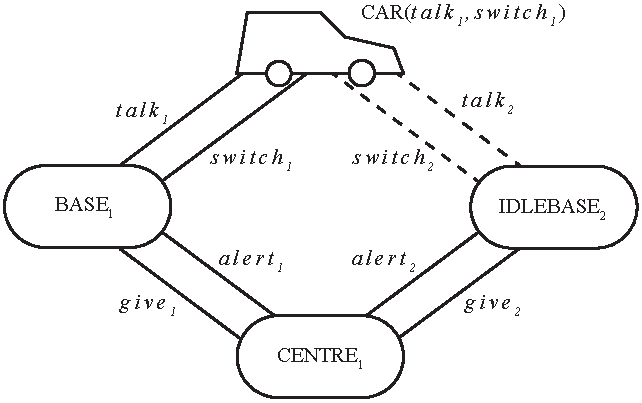
\includegraphics{handin-1-car-base-center-switching.pdf}
\caption{The system}
\end{center}
\end{figure}


\section{Exercise 3}
Here's an attempt at implementing the queue. It fails to maintain the order of the names in the queue but should work otherwise. Requesting a name is done over the channel q, while enqueueing happens over channel e. The last line takes care of enqueueing the three names initially in the queue.

\begin{equation}
\begin{split}
(v s, n_1, n_2, n_3)(!q(x) . s(n) . \overline{x} \langle n \rangle ) | !e(n) . \overline{s} \langle n \rangle | \\
\overline{e} \langle n_1 \rangle | \overline{e} \langle n_2 \rangle | \overline{e} \langle n_3 \rangle)
\end{split}
\end{equation}

\nocite{*}
\bibliographystyle{plain}
\bibliography{references}
\end{document}
\end{verbatim}
